\documentclass[12pt,a4paper]{article}
\usepackage{graphicx}
\usepackage[margin=2cm]{geometry} % Set the margins to 2cm on all sides
\usepackage{amsmath} % for advanced math typesetting
\usepackage{multicol}
\usepackage{enumitem}
\usepackage{url}
\usepackage{wrapfig}
\usepackage{array}
\usepackage{geometry}
\usepackage[table]{xcolor} % For shading cells

\usepackage{tikz}
\usetikzlibrary{shapes, arrows.meta, positioning, fit, backgrounds}


\begin{document}

% Cover Page
\begin{titlepage}
    \begin{center}
        \vspace*{1cm}

        
\includegraphics[width=0.75\textwidth]{UQLogo.jpg}
        
        \vspace{1.5cm}
        
        \textbf{\Large{School of Electrical Engineering and Computer Science}}
        
        \vspace{2.5cm}
        
        \textbf{\Large{REIT4841 THESIS  PROJECT PROPOSAL}}
        
        \vspace{0.5cm}

        \textbf{\Large{Low Cost Embedded Passive Bistatic Radar Detection}}
        
        \vspace{2cm}
        
        \textbf{Flynn Kelly}\\
        47418589\\
        
        Commenced: 17/02/2024 - S1 2024\\
        Mode of study: Full-time - Internal\\
        Supervisor: Dr Konstanty Bialkowski
        
        \vfill
        
        \vspace{0.8cm}
        
        \Large{1}
        
    \end{center}
\end{titlepage}

% Table of Contents
\tableofcontents
\clearpage

% Beginning of Sections

\section{Introduction}
This proposal introduces the theory, motivations and planned process for the creation of a low cost embedded bistatic passive radar detection system utilising a to be confirmed digital broadcast signal as the illuminator of opportunity. 

\subsection{Topic and Relevance}
Passive radar detection technology is a class of radar detection whereby the radar system does not emit any radiation. Instead, it uses existing electromagnetic signals in the environment, such as television or radio broadcasts, to detect and track objects. Passive radar can be bistatic, whereby the transmitter and receiver are separate, or multistatic, where there are multiple receivers. The technology has been around since the early 20th century, but has only recently become feasible due to advances in digital signal processing and computing \cite{INTRO2017}.
\par
\vspace{0.5cm} 
\noindent The technology has a number of advantages over traditional radar systems. It is covert, as it does not emit any radiation, and is therefore difficult to detect and directly jam, leading to a concentrated interest from defence cirlces \cite{DTSO2009}. It is also relatively cheap, as it does not require a dedicated transmitter and hence has less energy consumption. Conversely, it has a number of disadvantages, such as a lower signal-to-noise ratio, and a requirement for a relatively large amount of computational power to process the received signals \cite{INTRO2017}.
\par
\vspace{0.5cm} 
\noindent Bistatic passive radar detection has a wide range of applications centered around situational awareness, including air traffic control, border security, and environmental monitoring. Embedding the passive radar technology is a relatively new field buoyed by recent and increasing developments in computational power on Internet of Things (IoT) devices \cite{IOTpassiveRadar}. This project aims to reinforce and build on existing technology by creating a low-cost, modular, small-scale embedded passive radar detection system. Moreover, this project will also explore the possibility of scaling up this bistatic setup to a multistatic system, and the potential advantages and disadvantages of such. 

\par
\vspace{0.5cm} 
\noindent More specifically, the project will focus on streamlining the signal processing and computational requirements of both the line of sight signal and the reflected target signal onto a singular embedded setup, without PC hardware. This will be achieved by using a combination of existing embedded IoT hardware, and through using existing DSP (digital signal processing) and radar filtering algorithms. Initially, the illuminator of opportunitys explored are digital broadcast signals, and the target signal will be aerial vehicles. Noting that a range of other terrestrial illuminator signals can be utilised, often depending on the required use case, such as the tracking target and environment \cite{DABsignal}.

\subsection{Goals}
The primary goals of the project include the following, provided in order of logical progression;
\begin{itemize}
    \item Implement and investigate passive radar detection algorithms on high end computer architecture (PC) connected to SDR hardware and antenna for line of sight and target signal processing.
    \item Scaling down the passive radar detection system and associated algorithms to run on embedded IoT hardware, and investigate the computational and signal processing requirements, including the possible design of custom hardware such as peripheral functionality and printed circuit boards. A central feature of this specific goal is its ideally low cost nature.
    \item Verify functionality of low cost embedded passive radar detection system in a controlled environment against higher power computing results, and investigate the potential for scaling up to a multistatic system.
    \item Design and develop suitable housing for embdedded project implementation with ideal features such as modularity, portability and potential scaleability. 
\end{itemize}


\section{Background and Literature Review}

\subsection{Literature Review}
The below subsections reflect the neccessary research considerations for the project, and will be used to inform the project plan and optimize the implementation.

\subsubsection{Passive Radar Fundamentals}
The key and unique feature of passive radar is its utilisation of existing illuminators of opportunity, such as television or radio broadcasts, to detect and track objects. The technology has been around since the early 20th century, with modern interest accelerated due to the use passive radar systems on UHF TV signals and VHF FM radio tranmission systems in the 1980's \cite{FundamentalsPassiveRadar}. Equivalent terms used to describe passive radar include passive coherent location (PCL), and passive covert radar (PCR), parasitic radar, piggyback radar. Specifically, \textit{bistatic} radar refers to the distributed design of the transmitter and receiver, as opposed to classic \textit{monostatic} radar. As reflectd by Figure \ref{fig: topology} below, the turning parabolic of monostatic radar is able to receive both range and bearing of the signal echo, whereas passive bistatic radar measures time delay of the echos from the target, allowing doppler shift from the relative speed of the target to be measured.
\begin{figure}[htbp]
    \centering
    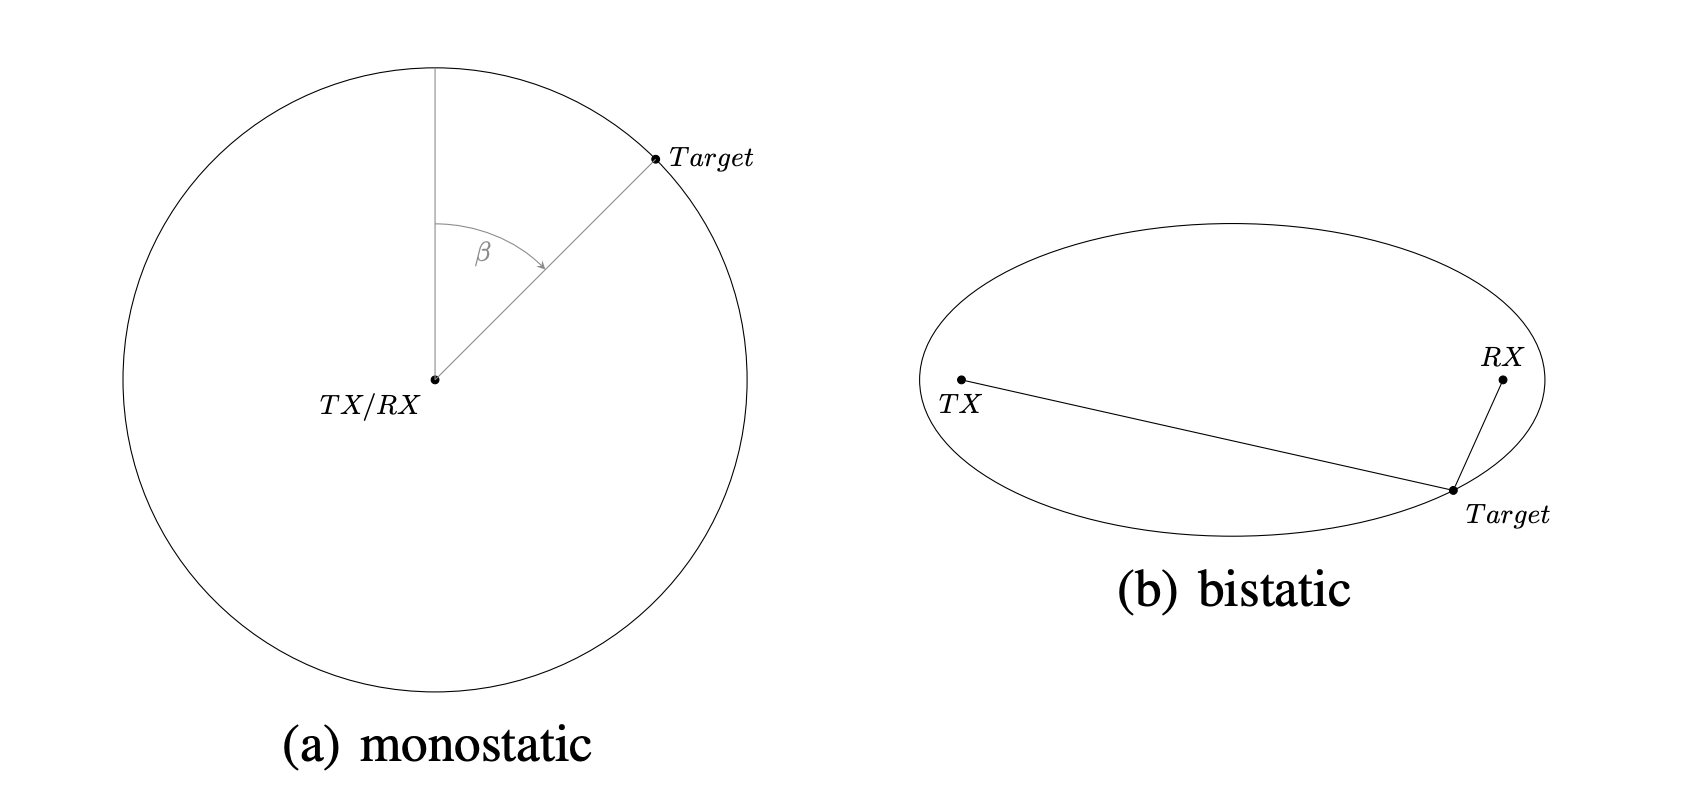
\includegraphics[width=0.8\textwidth]{monoBi.jpg}
    \caption{Monostatic (a) and bistatic (b) radar topologies \cite{IOTpassiveRadar}}
    \label{fig: topology}
\end{figure}
\par 
\vspace{0.5cm} 
\noindent The geometry of passive bistatic radar can be further explored and equations can be mapped accordingly, with the distance between the transmitter and receiver \textit{R} being determined by known quantities such as the baseline as reflected below in Figure \ref{fig:geometry}.

\begin{figure}[htbp]
    \centering
    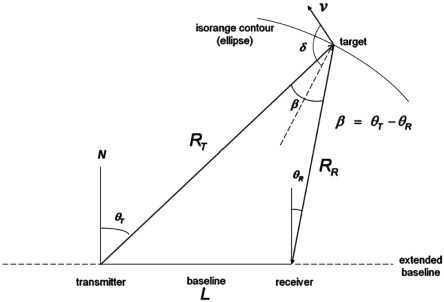
\includegraphics[width=0.8\textwidth]{geomPR.jpg}
    \caption{Bistatic radar geometry \cite{FundamentalsPassiveRadar}}
    \label{fig:geometry}
\end{figure}

\par \vspace{0.5cm} 
\noindent The bistatic range \( R_R \) is given by:
\begin{equation}
R_R = \frac{(R_T + R_R)^2 - L^2}{2(R_T + R_R + L \sin \theta_R)}
\end{equation}

\noindent The Doppler shift \( f_D \) is given by the rate of change of the bistatic range sum:
\begin{equation}
f_D = \frac{1}{\lambda} \frac{d}{dt}(R_T + R_R) \xrightarrow{} f_D = \frac{2v}{\lambda} \cos \delta \cos(\frac{\beta}{2})
\end{equation}
In the case of this project, both the TX (illuminator of opportunity) and the RX (embedded passive detection system) will be static, and the target will be moving, simplifying the mathematical calculations as much as possible, resulting in the cos version of equation 2 above. The Doppler shift will be used to determine the speed of the target as well as its relative directional motion, and the range will be used to determine the distance of the target from the receiver.

\par \vspace{0.5cm} 
\noindent Another important feature of bistatic passive radar systems is its performance which can be equated through the bistatic radar equation, which is equivalently derived as the monostatic radar equation \cite{FundamentalsPassiveRadar}. 
\vspace{0.5cm} 
\begin{equation}
    \frac{P_r}{P_n} = \frac{P_t G_t}{4\pi R_T^2} \cdot \sigma_B \cdot \frac{1}{4\pi R_R^2} \cdot \frac{G_r \lambda^2}{4\pi} \cdot \frac{1}{k T_0 B F}
\end{equation}
Where:
\begin{multicols}{2}
    \begin{itemize}
    \item \( P_r \) is the received target echo power.
    \item \( P_n \) is the receiver noise power.
    \item \( P_t \) is the transmit power.
    \item \( G_t \) is the transmit antenna gain.
    \item \( R_T \) is the transmitter-to-target range.
    \item \( \sigma_B \) is the target bistatic radar cross section.
    \item \( R_R \) is the target-to-receiver range.
    \item \( G_r \) is the receive antenna gain.
    \item \( \lambda \) is the signal wavelength.
    \item \( k \) is Boltzmann’s constant (\( 1.38 \times 10^{-23} \) JK\(^{-1}\)).
    \item \( T_0 \) is the noise reference temperature.
    \item \( B \) is the receiver effective bandwidth.
    \item \( F \) is the receiver effective noise figure.
    \end{itemize}
\end{multicols}
\noindent The denominator of the bistatic radar equation includes the term \( \frac{1}{R_T^2 R_R^2} \).This term implies that with omnidirectional antenna patterns, the contours of constant signal-to-noise ratio (SNR) are described by the equation \( R_T R_R = \text{constant} \), which represents Ovals of Cassini. In the case of directional antennas, these contours are altered. Moreover, the signal-to-noise ratio is minimized when the target is equidistant from the transmitter and receiver (\( R_T = R_R \)), and maximized when the target is closer to either the transmitter or receiver \cite{FundamentalsPassiveRadar}.

\par \vspace{0.5cm} 
\noindent Ideally this project would process just the target signal, however, that is an unrealistic expectation due to the presence of clutter. Clutter refers to unwanted signal that eminates from objects in the natural environment such as buildings, trees and ground \cite{zhang2023intelligent}. This process of target signal clutter suppression and its impact on range doppler mapping will be discussed later in the literature review.  

\subsubsection{Illuminators of Opportunity}
The illuminator of opportunity is the signal that is used to illuminate the target, and is the primary source of the signal that is received by the passive radar system. The illuminator of opportunity can be any signal that is transmitted through the air, such as television or radio broadcasts, and can be tailored to the specific requirements of the passive radar system. Griffiths and Baker outline the three key paramaters when selecting an illuminator \cite{INTRO2017}:
\begin{enumerate}[label=\arabic*.]
    \item The \textbf{Power Density} at the target: It refers to the strength of the signal (in Watts per square meter) that reaches the target area from the illuminator. Higher power density can improve detection performance due to a stronger return signal.
    \item The \textbf{Nature of the Waveform}: This includes the waveform's properties, such as bandwidth and modulation, which can affect the radar's resolution and ability to distinguish between targets and clutter.
    \item The \textbf{Coverage}: The spatial area over which the illuminator's signal is spread. Adequate coverage is essential to ensure the target is within the illuminator's effective range.
\end{enumerate}
Illuminator signals are not limited to terrestrial signals, and can also include signals from satellites, and can be tailored to the specific requirements of the passive radar system. The illuminator of opportunity primarily explored for this project is the DAB+ signal, and the target signal will be aerial vehicles - most likely in the form of civillian passenger jets. The DAB+ signal is a good option due to its high power density, and its relatively high bandwidth, which can be used to improve the radar's resolution and ability to distinguish between targets and clutter. Moreover, the geographical proximity of a DAB+ transmitter at Mt Cootha to the University of Queensland, St Lucia campus, making it a potentially ideal choice for the project. Another prospective digital illuminator signal is DVB-T (digital video broadcast - terrestrial), which is similar in its digital modulation to DAB, but provides increased bandwidth and signal power \cite{DVBsignal}. Furthemore, as shown by Yin et. al \cite{DVBnoise}, due to the relative complexity of  DVB visual signals, more signal processing steps can be required, which could exceed prospective hardware limitations of this project.

\par \vspace{0.5cm} 
\noindent A potential problem associated with the use of DAB as an illuminator is direct signal interference (DSI), with the effects being amplified in urban environments. Coleman et. al \cite{DABfeatures} explain that the sheer signal size of direct illuminator size relative to surveillance signal size results in a high level of DSI. They outline that the cross polarisation of the transmitted DAB signal can be utilised along with illuminator cancellation filtering to attain higher level suppression. The leakage of the illuminator signal into the target signal can be due to a range of factors including buildings, trees and other reflective items as highlighted by Palmer et. al \cite{DTSO2009}, specific filter arrangements will be explored later on.

\par \vspace{0.5cm} 
\noindent Typical characteristics of Australian DAB+ signals include frequency of just over 200MHz, bandwidth of approximately 1.5MHz, and a minimal output power of 10kW effective radiated power (ERP), consequently covering a large area \cite{DABfeatures}. These digital signals employ a modulation scheme called COFDM (coded orthogonal frequency division multiplexing), which is a form of multi-carrier modulation that is robust against multipath interference \cite{INTRO2017}. COFDM works by dividing the signal into multiple, simultaneous streams which are orthogonal to each other, modulated at a different frequency, maximising robust signal propogation. This is particularly useful in the context of passive radar, as it allows for the target and reference signal to be received by the passive radar system even if it has been reflected off multiple surfaces, such as buildings or trees.

\par \vspace{0.5cm} 
\noindent All of the above features result in DAB signals being condusive for ambiguity function performance (analyzed in further detail below). This can mainly be attributed to the relatively wide bandwidth of DAB enabling good resolution, constant DAB envelope stemming from COFDM protocol, and the multipath resistance \cite{DABambiguity}.
\subsubsection{Range Doppler Mapping}
Range doppler mapping is a technique used to determine the distance and relative velocity of targets by analyzing the frequency shift (Doppler shift) and time delay of the received signals after they bounce off the targets. The signal response of a target at a particular range and velocity can be predicted by the ambiguity function seen in equation 4 \cite{INTRO2017}. 
\begin{equation}
    \chi(\tau, f) = \int s_{reference}(t) s_{received}^*(t - \tau) e^{j2\pi f t} \, dt
\end{equation}
Where:
\begin{multicols}{2}
\begin{itemize}
\item \( \chi(\tau, f) \) is the ambiguity function.
\item \( \tau \) is the time delay.
\item \( f \) is the Doppler frequency.
\item \( s_1(t) \) is the transmitted signal.
\item \( s_2(t) \) is the received signal.
\item \( s_2^*(t - \tau) \) is the complex conjugate of the received signal, time-shifted by \( \tau \).
\item \( e^{j2\pi f t} \) is the complex exponential representing the Doppler shift.
\item The integral is taken over all time \( t \).
\end{itemize}
\end{multicols}
\noindent The ambiguity function can be plotted, thereby visualising resolution, sidelobe patterns and any discrepancies in range and doppler. This is especially important for passive bistatic radar, whereby waveforms are not explicitly designed for radar and the geometry also has an impact \cite{FundamentalsPassiveRadar}. Hughes visualises the geometry considerations and potential flaws of passive bistatic below in Figure \ref{fig:ambiguity}.

\begin{figure}[htbp]
    \centering
    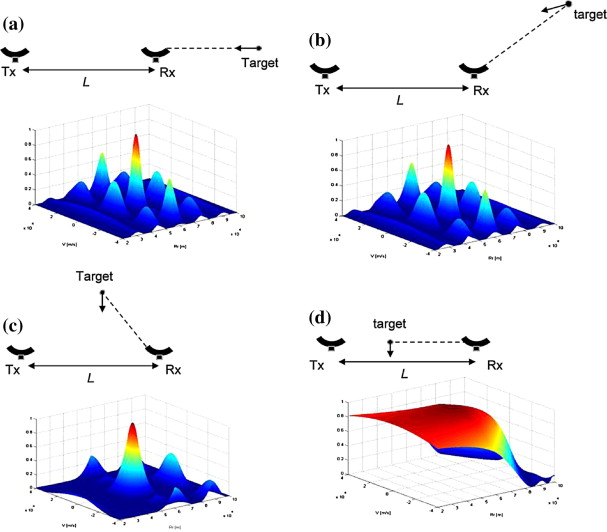
\includegraphics[width=0.7\textwidth]{ambiguity.jpg}
    \caption{Geometry and ambiguity function \cite{FundamentalsPassiveRadar}}
    \label{fig:ambiguity}
\end{figure}

\par \vspace{0.5cm} 
\noindent Understanding the link between geometric configuration and theoretical signal properties, the practical manifestation of the ambiguity function is range doppler mapping. As shown in Figure \ref{fig:rangeDoppler}, the map is a heat map and is derived with filters for noise minimsation, allowing for the visualisation of the target signal with minimal clutter. 
\begin{figure}[htbp]
    \centering
    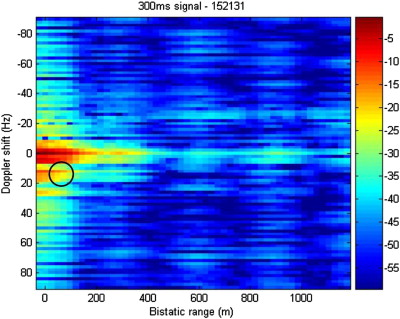
\includegraphics[width=0.6\textwidth]{rangeDoppler.jpg}
    \caption{Example of range doppler map for WiFi PBR \cite{FundamentalsPassiveRadar}}
    \label{fig:rangeDoppler}
\end{figure}
\par  
\noindent In the case of this project, the time delay will be utilised to calculate the bistatic range (x axis) and the Doppler shift will be used to calculate the relative velocity of the target (y axis). In summary, ambiguity function and subequent range doppler mapping will be vital for mapping the DAB+ signal characteristics for given geometry and motion of the surveilled target.

\subsubsection{Radio Hardware}
Given the low cost aims of this project, hardware cost will majorly impact the overall cost. Luckily, the proliferation of Software Defined Radio (SDR) has enabled low cost hardware modules enabling easy access to radio frequency (RF) signals \cite{SDRtheory}. The most popular SDR module is the RTL-SDR, which is a USB dongle that can be used to receive and decode a wide range of RF signals. The RTL-SDR is based on the Realtek RTL2832U chipset, and has a frequency range of 24MHz to 1.7GHz, and a bandwidth of 3.2MHz. The RTL-SDR is also relatively cheap, with a price of around \$40 AUD. The RTL-SDR is also compatible with a wide range of software, including MATLAB, and GNU radio \cite{SDRdongle}. Given the digital nature of the DAB+ signal, the direct reference signal and the target surveillance signal can in theory be sampled by a singular RTL2832U module as shown by Barrot et.al \cite{DABsingleRadar}. There are also a range of other off the shelf SDR options such as BladeRF and LimeSDR, which provide marginally improved performance at a substantial increase in cost and hardware \cite{SDRhardware}.  Regardless of sampling hardware architecture, based on previous studies and the nature of the DAB+ signal and modulation framework, a sampling rate of 2.048\,MS/s is prudent \cite{IOTpassiveRadar}. This hardware can be scaled up, accordingly providing a reference antenna and a surveillance antenna, as seen in Yardleys 2007 DAB receiver project \cite{antennaArchitecture}. On the contrary, as a potential extension, the use of a single antenna can be attempted with additional reconstruction processing required (providing lower hardware cost), this has been achieved by Barott and Engle \cite{DABsingleRadar}.

\subsubsection{IoT Architecture}
The IoT architecture in the scope of this project refers to the computational platforms utilised to undertake the digital signal processing which then maps to tracking and detection of the target. Existing studies have demonstrated the ability of off the shelf laptops \cite{FMlowCost}, and there is a few studies that use IoT platforms for FM signal processing \cite{IOTpassiveRadar}. The vital consideration when exploring hardware is the DSP requirements of the bistatic passive detection process (explored further in the next section).
\par \vspace{0.5cm} 
\noindent According to Schupbach et. al \cite{DABprocessingChain}, the broad scope capability requirements of the computational platform and associated processing can be grouped into signal acquisition, signal reconstruction and then the correlation function calculation. 
    
\noindent A possible IoT device that could be used, and has evidence of previous use as demonstrated by Moser et. al \cite{IOTpassiveRadar} is the Raspberry Pi platform, which despite having increased processing times, demonstrated its functionality. An alternate, higher powered choice in which Sednall demonstrated is the higher powered Nvidia Jetson, which includes faster processing times due to its quad core architecture \cite{FMlowCost}. The price for these options is \$60 compared to \$250 respectively. Ultimately, the choice of embedded IoT hardware for the project can be reduced to the trade off between low cost and processing power, and will be a key consideration in the project plan. Furthermore, there is possibility to design custom hardware to optimise for processing speeds and project cost, for example, a PCB extension utilising a Raspberry Pi with DSP IC chips and/or custom user buttons.



\subsubsection{Signal Processing and Algorithms} 

Broadly, the goal of the signal processing for this project is to extract a range doppler map from the received reference and surveillance signals. In order to achieve this, a range of steps are required to be undertaken. A range of literature exists for the signal processing of FM illuminator of opportunity signals, including Batches algorithm \cite{DSPfm}. However, given the nature of DAB and its COFDM modulation (explored above), filtering and synchronisation can be replaced with reconstruction of the surveillance signal \cite{DSPdab}. The use of a singular antenna is affirmed by Barott et. al \cite{DABsingleRadar} who utilised DAB passive radar to track micro-UAVs.

\begin{wrapfigure}{r}{0.6\textwidth} % This places the figure on the right and occupies 60% of the text width
    \centering
    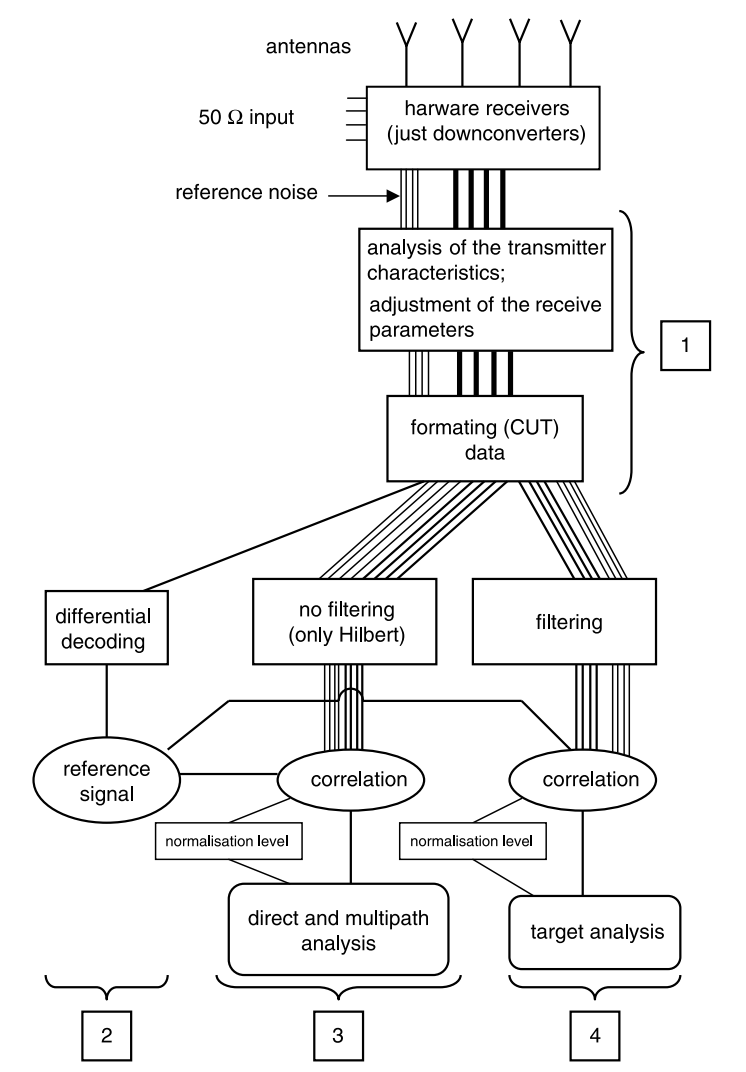
\includegraphics[width=0.45\textwidth]{DSPprocess.png}
    \caption{Main steps of signal processing \cite{detectionDABmodulation}}
    \label{fig:DSP}
\end{wrapfigure}

\par 
\noindent Figure \ref{fig:DSP} from Poullin \cite{detectionDABmodulation} shows the main steps of the required signal processing, which includes signal acquisition, reconstruction, and correlation. 

\par \vspace{0.5cm} 
\noindent The scope of this project involves branches 1 through 3, with target analysis representing a logical extension for a more complicated version of the project. 

\par \vspace{0.5cm} 
\noindent Once signal has been demodulated, according to Moser et. al, FFT the size of 2048 for the range domain and 512 for the doppler domain can be computed \cite{IOTpassiveRadar}, see Figure \ref{fig:FFT}. This can be combined with a decluttering chain, which can implement something along the lines of a weiner filter, or a matched filter, to remove unwanted signals from the range doppler map \cite{FundamentalsPassiveRadar}.

\noindent Logically, the step above relfects the most computationally intensive process of the project ... hence, considerations with regard to signal processing algorithms will need to be taken in order to keep the overall detection system low cost. Overall, Moser et. al provide a good introductory signal processing chain to utilise as a starting point \cite{IOTpassiveRadar}.

\begin{figure}[htbp]
    \centering
    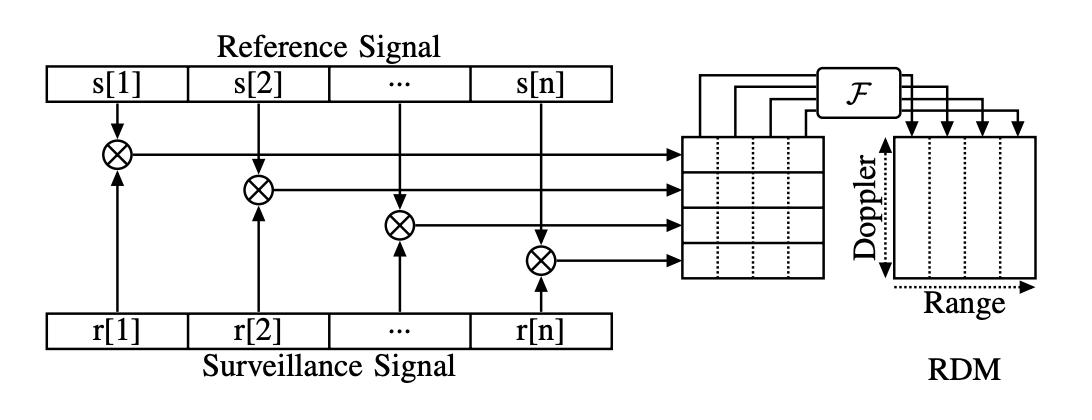
\includegraphics[width=0.8\textwidth]{FFT.png}
    \caption{Correlation and FFT for Range Doppler Mapping \cite{IOTpassiveRadar}}
    \label{fig:FFT}
\end{figure}

\subsubsection{Networking with Embedded Hardware} 
Given that the overall goal of this thesis project is to create a low cost, embedded passive radar detection system, valuable to consider how this would be visualised, be it wired via ethernet / UART to PC or wireless protocol. 

\subsection{Pilot Studies \& Existing PBR Technology}
As briefly alluded to in the above literature review, there is a plethora of existing research and pilot projects which utilise a range of hardware and illuminator of opportunity signals, including existing commercial products.

\subsubsection{Low-Cost Hardware}
The Swiss army have conduncted a very informative pilot study utilising both FM radio and DAB+ signals as illuminators of opportunity for an IoT based receiver design. Moser et. al explore the performance of a Raspberry PI GPU and CPU against a quad-core intel i7 equipped PC \cite{IOTpassiveRadar}. This paper also provided a good starting point for information regarding the difference in signal processing between digital (DAB+) and analogue (FM) illuminators of opportunity, including key characteristics as seen in Figure \ref{fig:signals} . 

\begin{figure}[htbp]
    \centering
    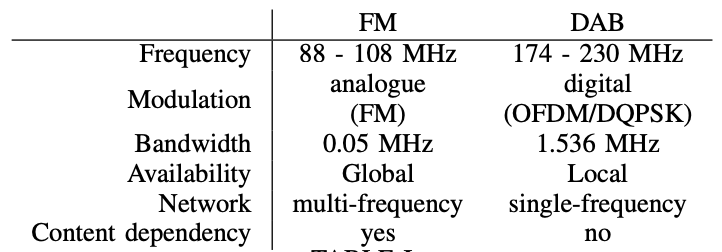
\includegraphics[width=0.4\textwidth]{digAnalog.png}
    \caption{Comparison Table - Analog vs Digital Signals \cite{IOTpassiveRadar}}
    \label{fig:signals}
\end{figure}

\par \vspace{0.5cm} 
\noindent Moser also provides a summary of the range doppler map generation process which itself is derived from Batches algorithm \cite{DSPfm}, including valuable performance measurements which indicate the efficacy of GPU processing over CPU processing.  The specific hardware utilised in Moser's paper was a Raspberry Pi v3; 1.2GHz Cortex A53 CPU along with a 400MHz VideoCore IV GPU. As of writing, the estimated cost to recreate this exact hardware (including SDR-RTL hardware) would be approximately \$100 AUD, representing a very low cost setup. Noting that hardware has also made significant advancements since the time of the paper (2019), with the Raspberry Pi v5 now available. The paper provides good hardware reference values for real-time processing limits of DAB frame computations, a key consideration area when optimizing for low cost hardware. 

\subsubsection{Illuminators of Opportunity}
Throughout the literature review, a range of papers exploring illuminator signals were explored, the DTSO report Written by Palmer, Palumbo, Van Cao, and Howard provides a good theoretical starting point. Whilst the scope of this proposal is confined to terrestrial illuminators (specifically digital audio), Palmer et. al highlight the wide range of use cases made available by other illuminators, including satellite signals and mobile phone signals. The report also provides a good overview of range doppler mapping, and target classification properties (despite the scope of this proposal not including target classification).

\begin{figure}[htbp]
    \centering
    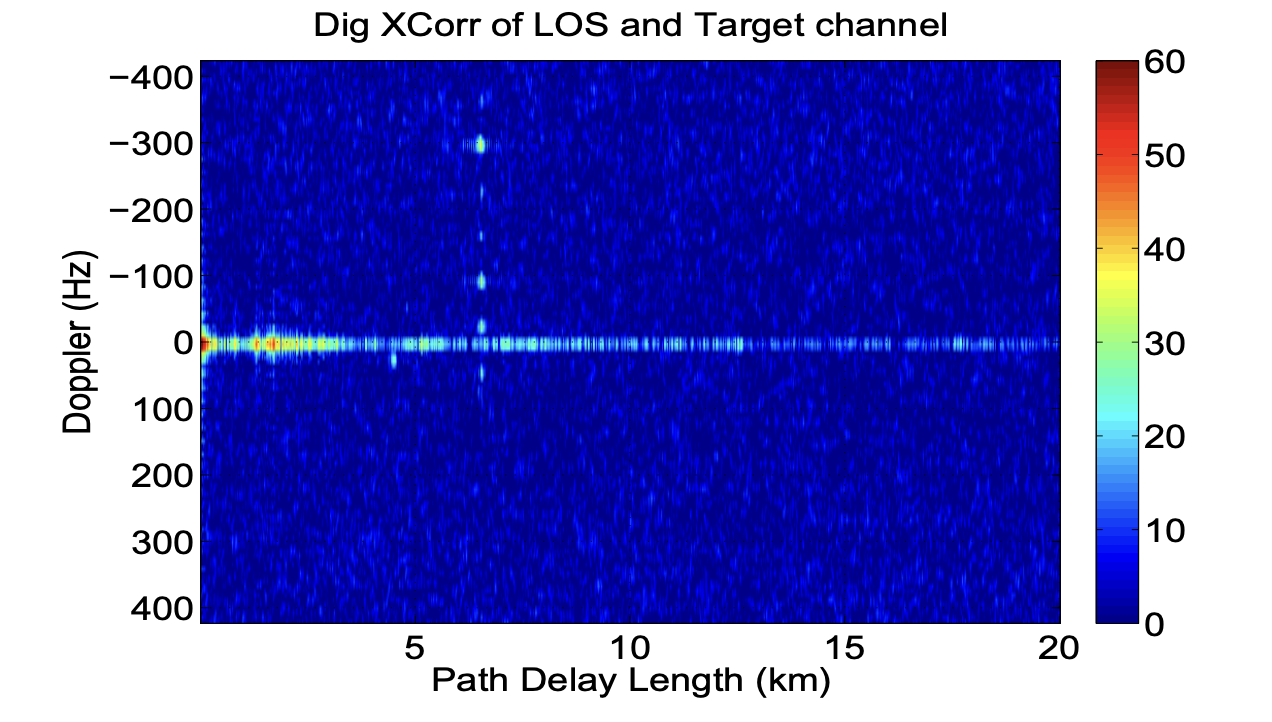
\includegraphics[width=0.7\textwidth]{movingTarget.jpg}
    \caption{RDM of target moving away from receiver \cite{DTSO2009}}
    \label{fig:rdm}
\end{figure}

\noindent As seen above in Figure \ref{fig:rdm}, in the .gif version of the image, the dot can be seen moving upwards (indicating motion away). This example also reflects effective de-cluttering of the RDM, a key step in passive tracking. An important consideration raised in this report is the edge case whereby the target moves along the bistatic ellipse as viewable in Figure \ref{fig: topology}, resulting in the doppler shift to be minimal and making tracking difficult.

\subsubsection{Signal Processing Architecture}
Once hardware and illuminator signal have been explored the next step is integrating these two and utilising / processing the sampled signals. A masters thesis by Sendall, was a very useful reference and pilot given its very similar scope, looking to optimise for cost without sacrificing too much computational performance \cite{FMlowCost}. A valuable takeway from this thesis was the intialisation and definition of project constraints, given the broadness of passive radar use cases and its optimisation areas it will be important to refine the scope scope and constraints.

\par \vspace{0.5cm} 
\noindent Sendall provides a hardware overview with valuable comparisons of the processor family, including performance/cost considerations of using DSP or FPGA architecture. Most valuably, he provides comprehensive detail about the signal processing chain, despite its analogue nature, it still provides a good starting point for shared obstacles such as de-cluttering and range doppler mapping.

\begin{figure}[htbp]
    \centering
    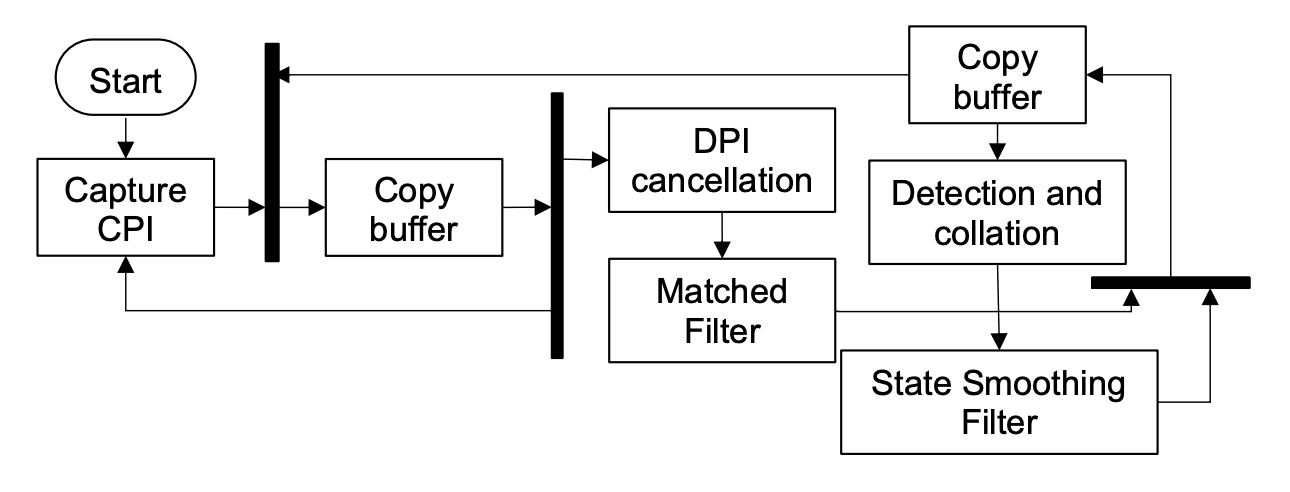
\includegraphics[width=0.7\textwidth]{filterChain.png}
    \caption{FM PBR Processing Chain \cite{FMlowCost}}
    \label{fig:fmChain}
\end{figure}

\par \vspace{0.5cm} 
\noindent Sendall's processing chain is based on his own literature review, and includes a comparison of different clutter minimisation filters, including adaptive filters, Wiener-Hoph filters and FDC filters. Valuably, Sendall outlines a range of evaluation metrics for the filter and hardware configuration including time complexity, floating point operations, maximum throughput, and power consumption (correlated to GPU occupancy).

\subsubsection{Commercial Technology}
Commercial industry has been developing passive radar for a number of years now, with the majority of such development occuring in the military space. Specifically,these innovations are in the realm of air sureveillance and can be either ground based or air based \cite{FundamentalsPassiveRadar}. Structurally, passive radar provides numerous advantages for defence applications including covert tracking due to the lack of a transmitter.
\par \vspace{0.5cm} 
\noindent \textbf{Lockheed Martin - SilentSentry:} One of the earliest commercial products utilising passive radar, the SilentSentry utilises analog illuminator signals with a dual horizontal linear phased array antenna to passively detect and track airborne targets \cite{DTSO2009}. It claims a detection range of up to 200km with an azimuth coverage of 60-360 degrees. Given the analog nature of the signals (FM and other terrestrial signals), it has a receiver for the direct line of sight signal and the echoed target signal before applying a signal processing algorithm.

\par \vspace{0.5cm} 
\noindent \textbf{Silentium Defence - Maverick-M:} Silentium is an Adelaide based company which produces man-portable low power, claiming to track small objects such as UAVs and drones. The Maverick-M utilises a bistatic configuration with a single receiver, and is able to track targets up to 100km away. The Maverick-M is also able to track multiple targets simultaneously, and is able to be used in a range of environments, including urban and mountainous areas \cite{Cilentium}. It utilises a range of ambient waves in the UHF and FM spectrums allowing maximul detection ability.

\subsection{Critique, Use and Evolution of Pilot Studies}
Given the nature of an undergraduate thesis project, it is unreasonable to assume revolutionary progress will be made. However, it is possible to utilise the cumulative knowledge and progress from existing technology and pilot projects to optimise a certain subject area. In the case of this embedded low-cost passive radar detection project, a lot of the same processes and technology will be utilised. This project will utilise the GPU process explored in section 2.2.1 whereby processing times are drastically faster than CPU processing. The project will also utilise the RTL-SDR hardware, and the DAB+ signal as the illuminator of opportunity. Furthermore, the FFT correlation calculations can be mimicked within the DSP. Importantly, the cost of hardware has decreased whilst computational power has simultaneously increased, hopefully allowing for a more efficient and cost effective iteration of Moser et. al implementation. Section 2.2.3 provided valuable performance metrics enabling a tested quantification method for this project, allowing comparison of hardware cost, configuration and performance. 

\section{Project Plan}
Intially, this this project can be broken into manageable milestones throughout both semesters allowing a progressively phased and consistent workload. In order to achieve completion by the end of the year, consistent communication with supervisor and adherence to self imposed deadlines will be vital. The project plan will be broken into the following sections:
\begin{enumerate}[label=\arabic*.]
    \item High level implementaiton of signal reception and processing on PC (Due end of week 13, semester 1, 2024)
    \item Selection and design of relevant hardware capable of handling the above signal processing algorithms (due end of week 8, semester 1, 2023)
    \item Application of signal reception and processing on embedded hardware (Due end of week 6, Semester 2, 2024)
    \item Implementation of RDM visualisation via chosen network protocol (Due end of week 8, Semester 2, 2024)
    \item Completion of final embedded design and housing along with thesis documentation (Due end of week 12, Semester 2, 2024)
\end{enumerate}


\begin{figure}[htbp]
    \centering
    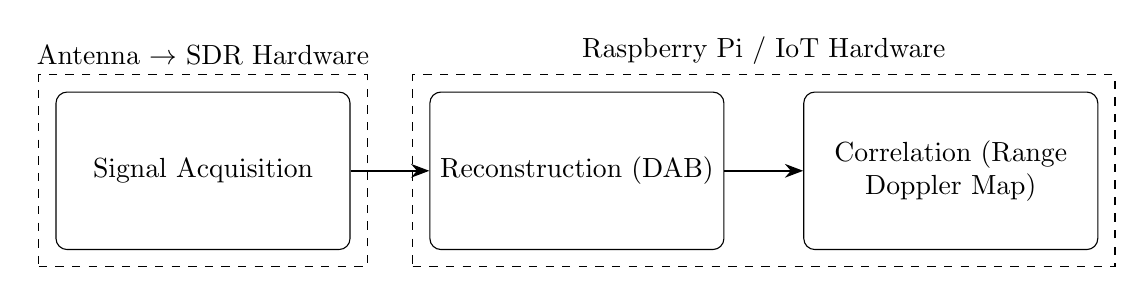
\begin{tikzpicture}[
        block/.style={
          rectangle,
          draw,
          text width=3.5cm,
          align=center,
          rounded corners,
          minimum height=2cm
        },
        line/.style={-Stealth, thick},
        dottedBox/.style={
          rectangle,
          draw,
          dashed,
          inner sep=6pt,
          label=above:#1
        }
    ]
    
    % Define the nodes
    \node[block] (signalAcq) {Signal Acquisition};
    \node[block, right=of signalAcq] (reconstruct) {Reconstruction (DAB)};
    \node[block, right=of reconstruct] (correlate) {Correlation (Range Doppler Map)};
    
    % Connect the nodes
    \draw[line] (signalAcq) -- (reconstruct);
    \draw[line] (reconstruct) -- (correlate);
    
    % Dotted boxes
    \node[dottedBox=Antenna $\rightarrow$ SDR Hardware, fit=(signalAcq)] {};
    \node[dottedBox=Raspberry Pi / IoT Hardware, fit=(reconstruct) (correlate)] {};
    
    \end{tikzpicture}
    \caption{Block diagram showing the high level hardware process}
    \label{fig:signal_processing_flow}
\end{figure}

\par \vspace{0.5cm} 
\noindent These milestones ensure that DSP and signal processing algorithms are implemented and tested in a non-hardware constrained environment, providing valuable benchmarks values. A visual overview of the required hardware and DSP interaction is provided above in Figure \ref{fig:signal_processing_flow}, putting the pending design choices required into context. Firstly, the passive bistatic tracking will be undertaken with PC software, while simultaneously in the background, embedded hardware will be analysed, chosen and configured with the goal of scaling the implementaiton onto it by early semester 2. The next milestone will be to extract the RDM and visualise it through an optimal communication / network protocol, allowing viewing of tracking without associated signal processing. Finally, the thesis project will be written up and the final embedded passive radar hardware will be housed, resulting in a small-scale final product.

\subsection{Milestone 1 - Implementation of Signal Reception and Processing Algorithms on PC Hardware}
The initial phase of the project will involve a further comprehensive review of the passive bistatic DSP literature, with the selection and finalising of algorithms. The signal acquisition process will be tested and implemented with the RTL-SDR module, and the processing will be tested through PC hardware (specifically M1 macOS). The concept behind this testing is for familiarisation with the decluttering process and correlation processing. Resources required for this milestone include the RTL-SDR dongle, LPDA antenna, MATLAB and/or similar software to undertake the signal processing. The following sub tasks comprise this milestone:
\begin{multicols}{2}
    \begin{itemize}
    \item Finalisation of proposal with enhanced DSP detail and references
    \item More comprehensive literature review with declutter algorithm comparison and exploration of sureveillance signal remodulation.
    \item Install neccessary radio software on device such as spektrum and welle.io
    \item Configure LPDA and SDR dongle
    \item Read in Mt Cootha DAB+ signal through RTL-SDR dongle, noting consellation diagram features
    \item Install neccessary signal processing software - MATLAB???? 
    \item Process echoed surveillance signal and test demodulation and reconstruction algorithm
    \item Implement correlation FFT algorithm
    \item Generate / visualise RDM
    \item Calculate relevant signal processing evalutation metrics such as processing time, real time limit, and DAB frame througput.
    \end{itemize}
\end{multicols}

\subsection{Milestone 2 - Selection/Design of Embedded Hardware Optimised for Cost} 
Simultaneously whilst the signal processing and range doppler mapping processing is occuring on higher level hardware, this milestone aims to evaluate and select hardware whihc can undertake said processing but be optimised for low cost and size. Hence it primarily encompasses evaluation and consideration of any requried custom features that may arise.
\begin{multicols}{2}
    \begin{itemize}
    \item Literature review of parrallel architecture use (ie. FPGA)
    \item Selection and comparison of at least three potential IoT devices / architectures with considerations around cost and DSP evaluation metrics
    \item Choose architecture; ie. Raspberry Pi v5
    \item Consider customiseable functionality ie. a track target user input
    \item Completion of hardware schematic which includes RTL-SDR module and system interfacing
    \item Selection of programming language - c, circuit py???
    \item Flash hardware and test through sampling DAB signal, etc. 
    \end{itemize}
\end{multicols}

\subsection{Milestone 3 - Application of Signal Processing Algorithms and Tracking on Embedded Hardware} 
Dependent on the completion of each of the previous milestone, this milestone represents the crux of this thesis, the implementation of passive bistatic radar tracking on low cost hardware. The complete tracking pipeline should be completed in this stage from processing the surveillance signal to the generation of range doppler maps, this will be completed provided the following outcomes are met:
\begin{multicols}{2}
    \begin{itemize}
    \item Implement selected algorithms in software on the embedded device
    \item Utilise the embedded equivalent of signal data structures from the PC implementation
    \item Implement appropriate control flow on embedded device and flash the chained DSP algorithms
    \item Test the ability of the device to generate a generic RDM (through serial connection to PC)
    \item Test the device through tracking a reasonably close by civillian airliner 
    \item Flash hardware and test through sampling DAB signal, etc. 
    \end{itemize}
\end{multicols}

\subsection{Milestone 4 - Communication of Tracking Data / RDM From Embedded Hardware} 
This milestone will involve the implementation of a network / communcation protocol to share the range doppler map from the embedded hardware to a PC. If the embedded hardware is something like a Raspberry Pi, thisn will enable a more user friendly and visual representation of the tracking data, moreover it also allows for the future potential of scaling up to a multistatic system. The below steps should be considered and implemented;
\begin{multicols}{2}
    \begin{itemize}
    \item Explore an appropriate communication protocol given the size of RDM data, UDP, MQTT, etc.
    \item Evaluate potential network configurations, ie UQ Wifi, Traffic Monitoring Network
    \item Generate RDM data into serialized transmittable format such as a JSON file
    \item Implement required code on embedded side for transmission and visualisation software on the PC side.
    \end{itemize} 
\end{multicols}

\subsection{Milestone 4 - Complete Embedded Design and Housing, Final Thesis Documentation} 
At this stage of the process all the signal processing, communication and tracking will be undertaken on the hardware. The goal at this point will be to finalise a design which would enable rigid performance and portability. The final thesis documentation will also be completed at this stage. The following steps should be undertaken:
\begin{multicols}{2}
    \begin{itemize}
    \item Selection of relevant casing for the embedded
    \item Potential implementation of battery pack
    \item Generation of a user manual for the systems
    \item Write up of the final thesis documentation
    \end{itemize} 
\end{multicols}

\newpage
\section{Risk Assessment}

\begin{table}[htbp]
    \centering
    \caption{Potential Risks Involved with Project}
    \vspace{0.5cm}
    \begin{tabular}{|>{\raggedright\arraybackslash}p{3cm}|p{3cm}|p{6cm}|}
    \hline
    \rowcolor{gray!30} \textbf{Risk} & \textbf{Probability} & \textbf{Method of Prevention} \\
    \hline
    Signal Reliability & Low & DAB+ very reliable signal as the illuminator \\
    \hline
    Hardware Failure & High & Regularly test and maintain equipment, have backup components \\
    \hline
    Thermal Management Issues & High & Design efficient heat dissipation systems for the hardware - should be considered in design \\
    \hline
    Software Bugs & High & Follow best coding practices, regularly update and patch software \\
    \hline
    Environmental Conditions & Medium & Use rugged components and casing suitable for varying weather conditions \\
    \hline
    \end{tabular}
    \label{table:risks}
    \end{table}
    

\section{Ethics Assessment}
Given the technical nature of the project, which strictly involves the use of radar hardware/software for signal processing and does not include any human subjects, human data, or animals, the ethical considerations are significantly minimal. There are no planned interventions or interactions with human participants, and as such, there is no need for human ethics approval or the consideration of issues such as consent, privacy, and confidentiality that are typically associated with human subject research.


% References (You will need to use BibTeX to manage your references)
% The bibliography style can be changed to suit your needs
\newpage
\addcontentsline{toc}{section}{References} % Adds "References" to your TOC
\bibliographystyle{plain}
\bibliography{references}

\end{document}
